\section{SQL Queries}
Af Kasper\\\\
Alle metoder til at behandle SQL statements til vore MySQL database findes i DataAccessObject-klassen. Vi benytter os af PreparedStatements for at gøre systemet hurtigere og mere stabilt, og for at sikre os mod SQL-injection angreb.\\
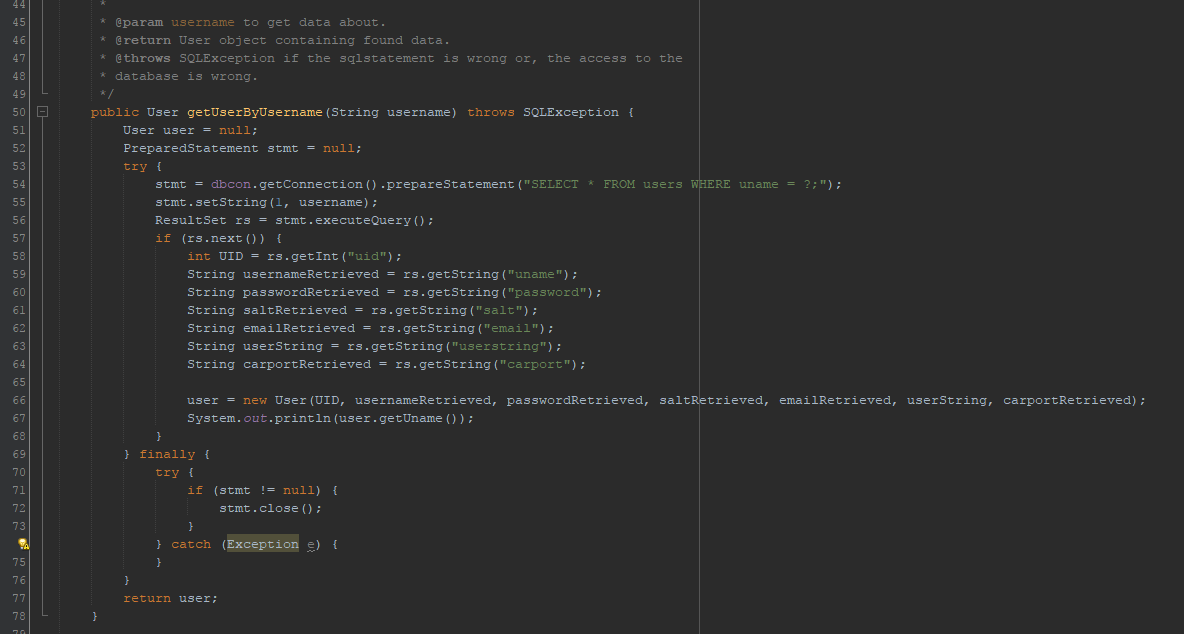
\includegraphics[width=\textwidth]{sqlstatement}
PreparedStatements indsætter de strings der bliver givet med til metoden der hvor spørgsmålstegnene står. Dette er ligegyldigt hvad der står i den string der kommer med, derfor bliver SQL-injection umuliggjort her.\\
MySQL-Databasen er opbygget specifikt efter vores egne behov. Derfor er den ikke særlig fleksibel. Dog er tabellen med dele til carporten bygget op så både skruer, brædder, søm osv. kan være i samme tabel. dette er gjort ved at definere forskellige dele-id'er som markerer forskellige typer materialer.\\
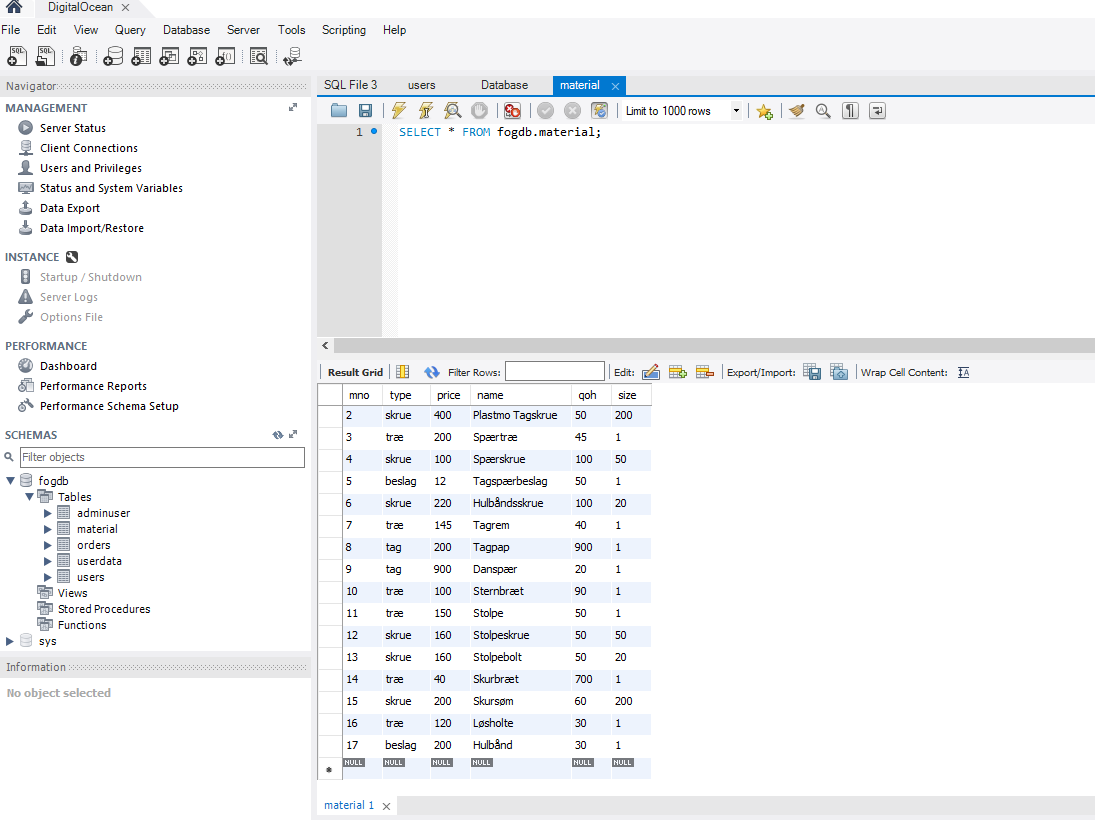
\includegraphics[width=\textwidth]{partssql}